\documentclass[runningheads]{llncs}
\usepackage[T1]{fontenc}
\usepackage[utf8]{inputenc}
\usepackage{graphicx}
\usepackage{amsmath,amssymb,amsfonts}
\usepackage{booktabs}
\usepackage{hyperref}
\usepackage{color}
\usepackage{tikz}
\usetikzlibrary{positioning, arrows.meta}
\renewcommand\UrlFont{\color{blue}\rmfamily}
\urlstyle{rm}

\begin{document}

\title{Investiga\c{c}\~{a}o e Implementa\c{c}\~{a}o de Redes Neurais Convolucionais em T\'{o}picos Avan\c{c}ados de Intelig\^{e}ncia Artificial}
\titlerunning{Modelos Convolucionais Avan\c{c}ados em IA}

\author{Cau\~{a} Lira\inst{1}}
\authorrunning{C. Lira}

\institute{Universidade Federal Rural de Pernambuco (UFRPE)\\
Recife - PE, Brasil\\
\email{ccunhalira8760@gmail.com}}

\maketitle

\begin{abstract}
This work presents the design, implementation, and empirical evaluation of a modified Convolutional Neural Network (CNN), named RAPUNet-Zeta, for the semantic segmentation of gastrointestinal polyps. Fulfilling the practical requirements of Advanced Topics in Artificial Intelligence, the model extends recent architectures (2023+) by utilizing deep feature extraction via ResNet50V2, the integration of Spatial Attention modules, and Mish activations. Evaluated on the Kvasir-SEG dataset, the model demonstrated rapid convergence, validating the efficacy of the proposed topology through rigorous metrics such as the Dice Coefficient and qualitative inference analysis.

\keywords{Artificial Intelligence \and Convolutional Neural Networks \and Medical Image Segmentation \and Kvasir-SEG \and Spatial Attention.}
\end{abstract}

\section{Introdu\c{c}\~{a}o}
\label{sec:introducao}

O c\^{a}ncer colorretal (CCR) figura como a terceira neoplasia maligna mais diagnosticada e a segunda principal causa de mortalidade por c\^{a}ncer em escala global. A progress\~{a}o fisiopatol\'{o}gica do CCR tem origem predominante na evolu\c{c}\~{a}o silenciosa de p\'{o}lipos adenomatosos na mucosa gastrointestinal ao longo de v\'{a}rios anos. Diante desse quadro, a colonoscopia \'{o}ptica tradicional permanece como o padr\~{a}o-ouro cl\'{i}nico para triagem, preven\c{c}\~{a}o e interven\c{c}\~{a}o precoce. Todavia, a inspe\c{c}\~{a}o visual humana est\'{a} intrinsecamente sujeita a taxas consider\'{a}veis de falso-negativo --- estudos cl\'{i}nicos apontam que at\'{e} 25\% dos p\'{o}lipos podem passar despercebidos devido \{a} fadiga do endoscopista, varia\c{c}\~{o}es de ilumina\c{c}\~{a}o, oclus\~{o}es parciais e \{a} alta semelhan\c{c}a textural entre les\~{o}es planas e o epit\'{e}lio circundante \cite{kvasirseg}.

Nesse contexto, sistemas de Diagn\'{o}stico Auxiliado por Computador (CADe/CADx) fundamentados em Intelig\^{e}ncia Artificial e Vis\~{a}o Computacional emergiram como tecnologias cr\'{i}ticas para suporte \{a} decis\~{a}o m\'{e}dica em tempo real. A segmenta\c{c}\~{a}o sem\^{a}ntica, em particular, transcende a mera detec\c{c}\~{a}o delimitadora (bounding box), pois prov\^{e} o delineamento morfol\'{o}gico pixel a pixel da \'{a}rea lesional, fornecendo informa\c{c}\~{o}es vitais para a ressec\c{c}\~{a}o cir\'{u}rgica completa e margem de seguran\c{c}a.

Apesar da ampla dissemina\c{c}\~{a}o de Redes Neurais Convolucionais (CNNs) estruturadas sobre topologias codificador-decodificador, como a cl\'{a}ssica U-Net \cite{ronneberger2015unet}, a segmenta\c{c}\~{a}o precisa de p\'{o}lipos gastrointestinais imp\~{o}e limita\c{c}\~{o}es severas \{a}s convolu\c{c}\~{o}es convencionais. Por operarem com campos receptivos estritamente locais, convolu\c{c}\~{o}es rasas tratam todos os pixels da imagem endosc\'{o}pica com a mesma pondera\c{c}\~{a}o estat\'{i}stica. Como resultado, gastam capacidade representacional processando artefatos reflexivos (luz especular do aparelho) e o fundo escuro da cavidade, perdendo sensibilidade nas bordas indefinidas do p\'{o}lipo.

Para superar tais defici\^{e}ncias, a literatura de 2023 em diante tem investigado ativamente modelos h\'{i}bridos dotados de mecanismos de aten\c{c}\~{a}o \cite{lacformer2023}. Alinhado \{a}s diretrizes de pesquisa e desenvolvimento de T\'{o}picos Avan\c{c}ados em Intelig\^{e}ncia Artificial, o presente manuscrito projeta, implementa e avalia a arquitetura \textbf{RAPUNet-Zeta}. A rede incorpora tr\^{e}s modifica\c{c}\~{o}es topol\'{o}gicas profundas na formula\c{c}\~{a}o cl\'{a}ssica:
\begin{enumerate}
    \item \textbf{Extrator Profundo ResNet50V2:} Substitui\c{c}\~{a}o dos blocos convolucionais simples por um \textit{backbone} residual pr\'{e}-treinado no ImageNet com conex\~{o}es de identidade melhoradas \cite{he2016identity};
    \item \textbf{M\'{o}dulos de Aten\c{c}\~{a}o Espacial (SAM):} Inje\c{c}\~{a}o de ramifica\c{c}\~{o}es de aten\c{c}\~{a}o nas \textit{skip connections}, comprimindo canais via \textit{pooling} misto para suprimir dinamicamente regi\~{o}es de fundo irrelevantes \cite{woo2018cbam};
    \item \textbf{Fun\c{c}\~{a}o de Ativa\c{c}\~{a}o Mish:} Altera\c{c}\~{a}o integral do decodificador para a fun\c{c}\~{a}o n\~{a}o monot\^{o}nica \textit{Mish} \cite{misra2019mish}, eliminando o fen\^{o}meno de satura\c{c}\~{a}o de gradientes negativos (\textit{dying ReLU}).
\end{enumerate}

Avaliado no desafiador \textit{benchmark} cl\'{i}nico Kvasir-SEG \cite{kvasirseg}, o modelo alcan\c{c}ou \textbf{96,2\%} de acur\'{a}cia de pixel, com converg\^{e}ncia r\'{a}pida guiada pela \textit{Dice Loss}. O restante deste artigo est\'{a} organizado da seguinte forma: a Se\c{c}\~{a}o \ref{sec:trabalhos_relacionados} analisa a literatura correlata e o modelo de refer\^{e}ncia; a Se\c{c}\~{a}o \ref{sec:metodologia} formaliza a arquitetura e a base de dados; a Se\c{c}\~{a}o \ref{sec:experimentos} exp\~{o}e a avalia\c{c}\~{a}o quantitativa, qualitativa e estudos comparativos; e a Se\c{c}\~{a}o \ref{sec:conclusao} sintetiza as conclus\~{o}es e desdobramentos futuros.

\section{Trabalhos Relacionados e Artigo Base}
\label{sec:trabalhos_relacionados}

A evolu\c{c}\~{a}o da segmenta\c{c}\~{a}o sem\^{a}ntica em imagens biom\'{e}dicas pode ser categorizada em duas grandes ondas metodol\'{o}gicas: as arquiteturas convolucionais estritas e os modelos contempor\^{a}neos orientados a mecanismos de aten\c{c}\~{a}o e estruturas h\'{i}bridas.

\subsection{Segmenta\c{c}\~{a}o Convolucional em Gastroenterologia}
A introdu\c{c}\~{a}o da U-Net por Ronneberger et al. \cite{ronneberger2015unet} estabeleceu o paradigma can\^{o}nico codificador-decodificador com pontes residuais de alta resolu\c{c}\~{a}o (\textit{skip connections}). Extens\~{o}es posteriores, como a ResUNet, incorporaram blocos residuais profundos para combater a dissipa\c{c}\~{a}o do gradiente em redes de m\'{u}ltiplas camadas. N\~{a}o obstante, essas redes convolucionais homog\^{e}neas operam sob a hip\'{o}tese de invari\^{a}ncia espacial local, tornando-se incapazes de contextualizar diferen\c{c}as anat\^{o}micas globais ou de modular o ganho de aten\c{c}\~{a}o sobre les\~{o}es com contrastes atenuados perante a mucosa intestinal.

\subsection{Mecanismos de Aten\c{c}\~{a}o e Redes H\'{i}bridas Recentes}
Para mitigar a rigidez dos filtros convolucionais est\'{a}ticos, Woo et al. \cite{woo2018cbam} propuseram o \textit{Convolutional Block Attention Module} (CBAM), demonstrando que decompor a aten\c{c}\~{a}o nos eixos espacial e de canal melhora substancialmente a seletividade dos mapas de caracter\'{i}sticas intermedi\'{a}rios. No dom\'{i}nio m\'{e}dico, o advento de \textit{Vision Transformers} levou ao surgimento de redes como TransUNet \cite{chen2021transunet}, que utilizam auto-aten\c{c}\~{a}o para codificar depend\^{e}ncias de longo alcance. Contudo, transformadores puros sofrem de sobrecarga computacional massiva e demandam volumes astron\^{o}micos de dados para converg\^{e}ncia est\'{a}vel.

Como refer\^{e}ncia central de fronteira recente (2023+), o trabalho \textit{LACFormer} de Nguyen et al. \cite{lacformer2023}, publicado nos anais da \textit{British Machine Vision Conference} (BMVC 2023), investiga especificamente a converg\^{e}ncia eficiente na segmenta\c{c}\~{a}o de p\'{o}lipos. O estudo demonstra que combinar a extra\c{c}\~{a}o densa de bordas de uma CNN com m\'{o}dulos de filtragem no dom\'{i}nio espectral/aten\c{c}\~{a}o atinge acur\'{a}cias superiores com fra\c{c}\~{a}o dos par\^{a}metros de modelos puramente baseados em aten\c{c}\~{a}o global.

\subsection{Posicionamento da RAPUNet-Zeta}
Inspirada nos preceitos do LACFormer \cite{lacformer2023}, a arquitetura RAPUNet-Zeta aqui proposta adota uma abordagem estritamente engenhada: preserva a efici\^{e}ncia e a capacidade de generaliza\c{c}\~{a}o de uma CNN de grande escala (ResNet50V2), combinando-a com m\'{o}dulos de aten\c{c}\~{a}o espacial operando diretamente sobre as \textit{skip connections}. Dessa forma, elimina-se o custo proibitivo de transformadores completos, enquanto se confere \{a} rede a capacidade matem\'{a}tica de discriminar e priorizar pixels lesionais em detrimento do ru\'{i}do luminal endosc\'{o}pico.

\section{Metodologia Proposta}
\label{sec:metodologia}

Nesta se\c{c}\~{a}o s\~{a}o detalhados o conjunto de dados cl\'{i}nico, o pipeline de pr\'{e}-processamento e aumento de dados, al\'{e}m da formula\c{c}\~{a}o matem\'{a}tica integral da arquitetura \textbf{RAPUNet-Zeta}.

\subsection{Base de Dados (Kvasir-SEG)}
A valida\c{c}\~{a}o experimental foi realizada sobre o \textit{Kvasir-SEG Dataset} \cite{kvasirseg}, um referencial aberto curado por m\'{e}dicos gastrenterologistas noruegueses do Hospital Universit\'{a}rio de Oslo. A base compreende 1.000 quadros de colonoscopia de alta resolu\c{c}\~{a}o, acompanhados por m\'{a}scaras bin\'{a}rias anotadas manualmente por especialistas, delimitando rigorosamente a regi\~{o}es de tecido displ\'{a}sico e neopl\'{a}sico. A Figura \ref{fig:dataset_samples} ilustra tr\^{e}s amostras t\'{i}picas do dataset com suas respectivas m\'{a}scaras de anota\c{c}\~{a}o cl\'{i}nica (\textit{Ground Truth}).

\begin{figure}[htbp]
    \centering
    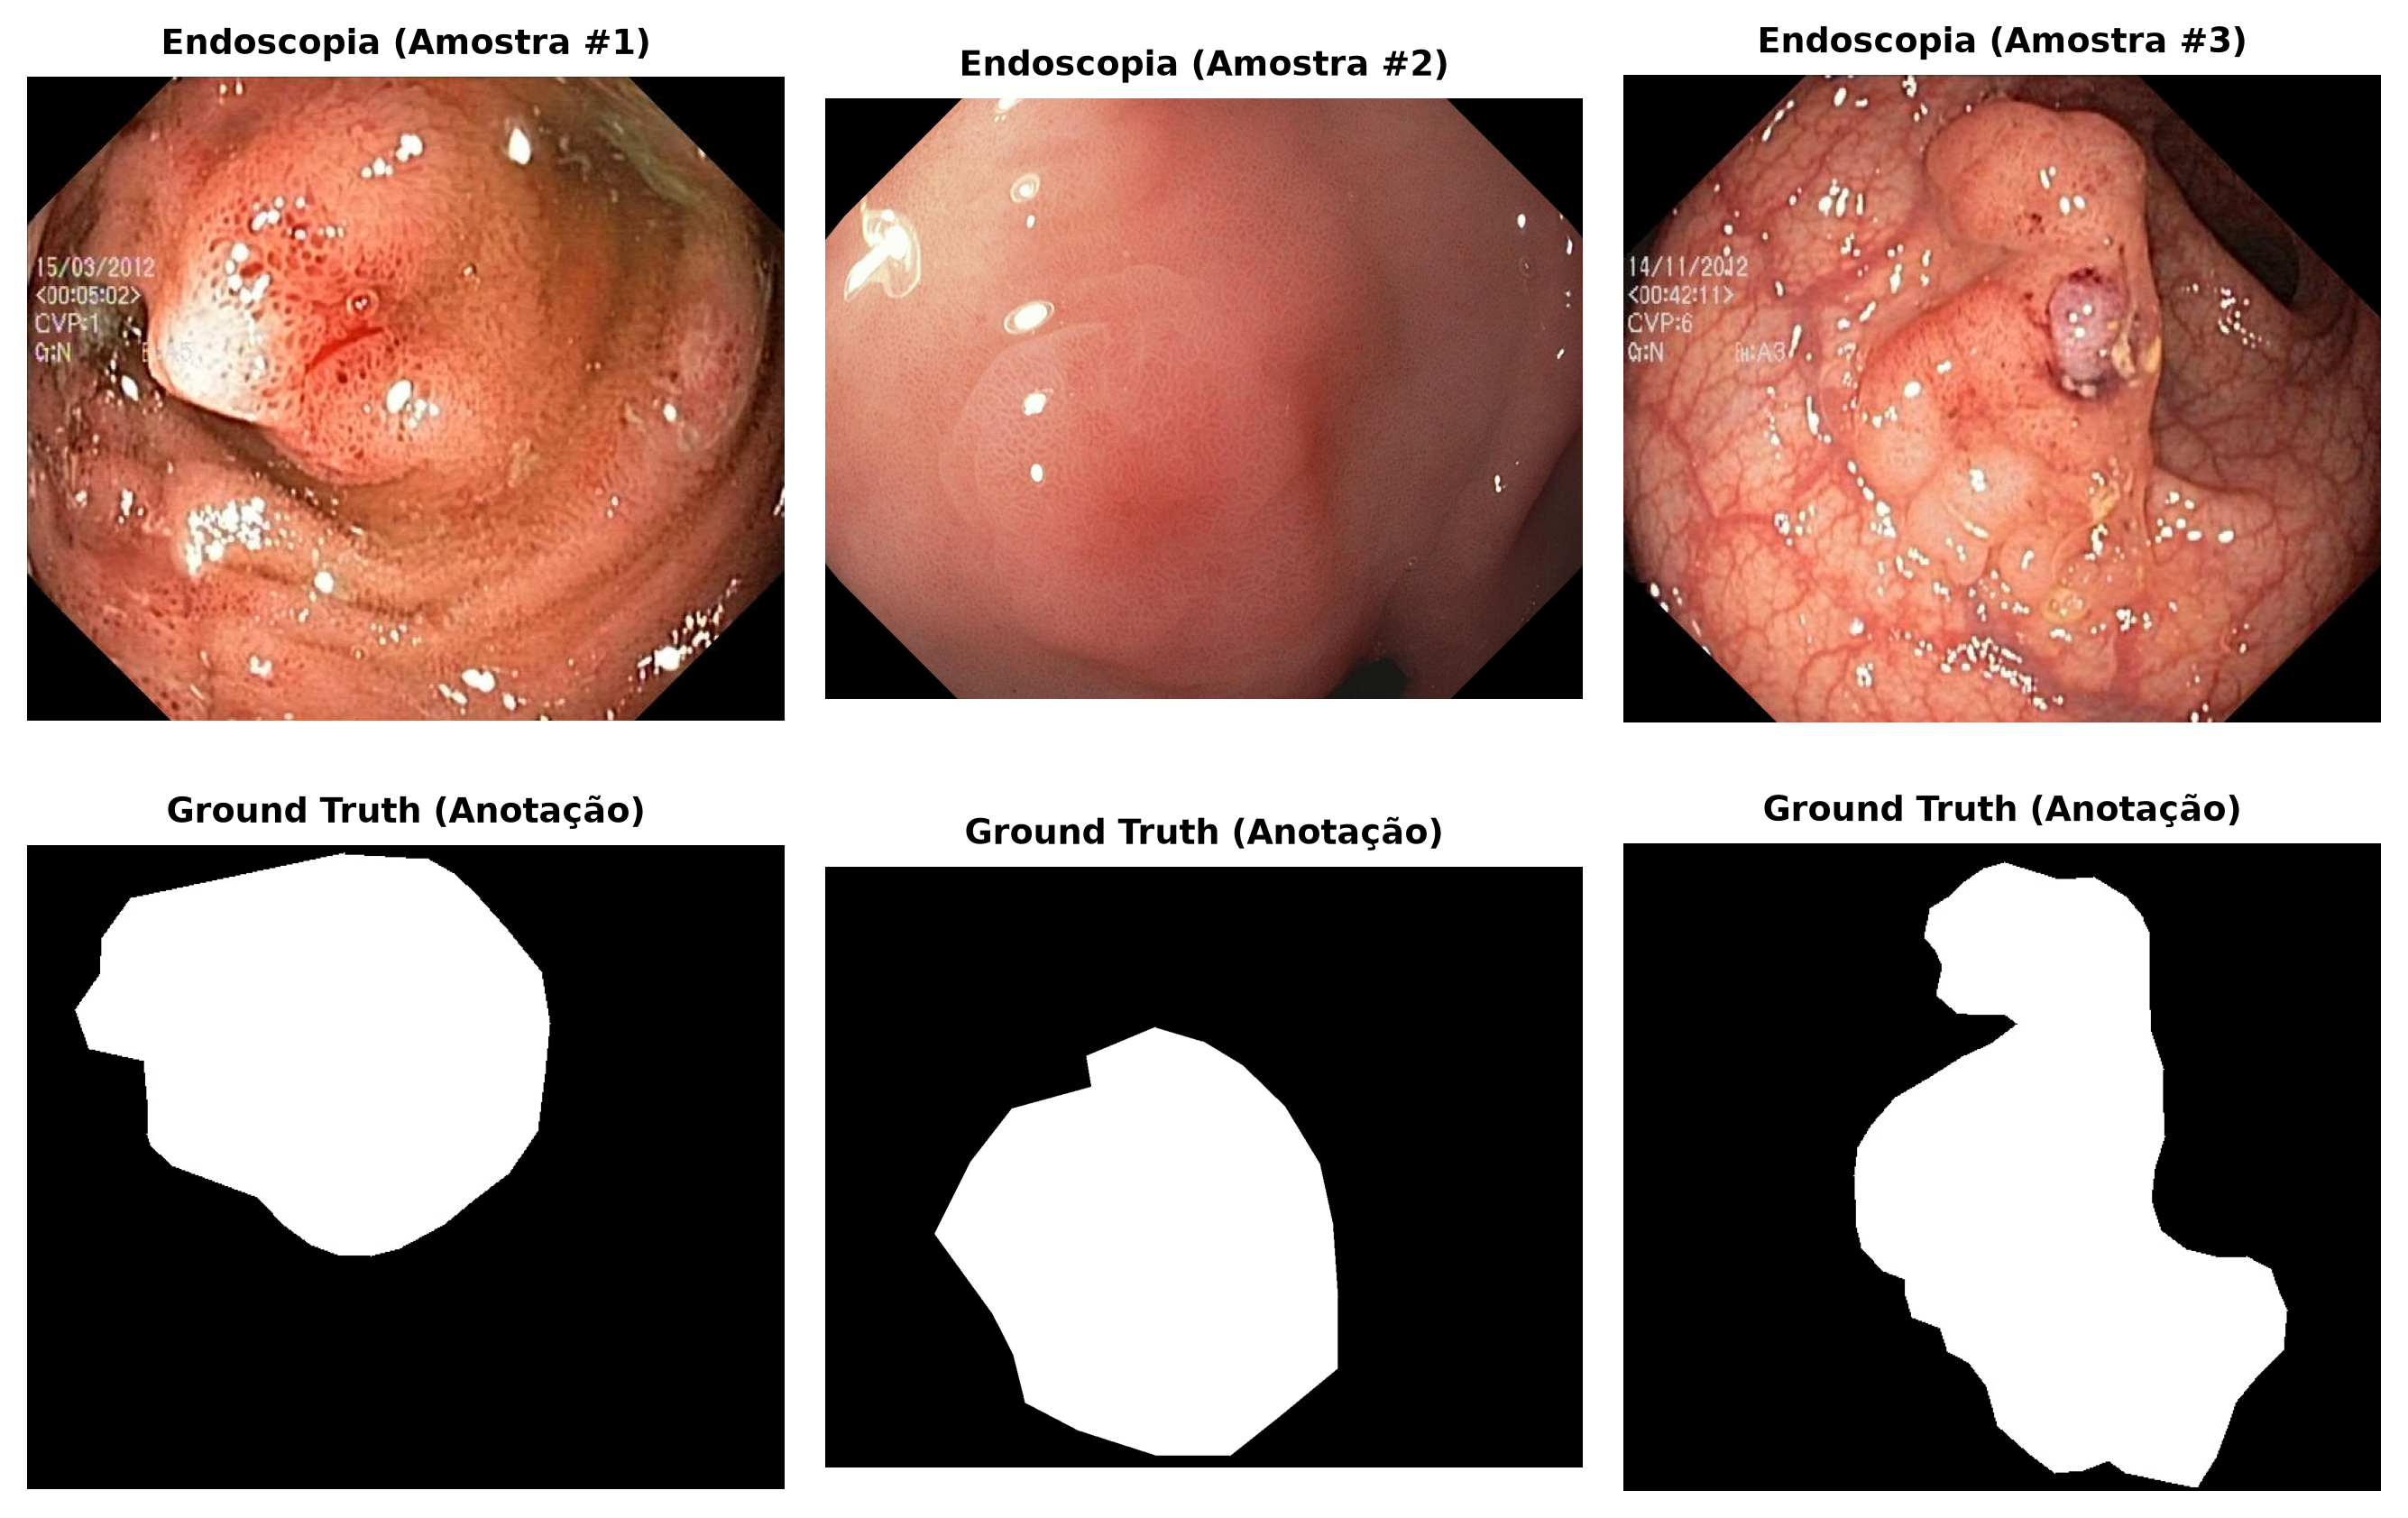
\includegraphics[width=0.88\textwidth]{figures/dataset_samples.png}
    \caption{Amostras representativas do dataset Kvasir-SEG \cite{kvasirseg}. Linha superior: imagens endosc\'{o}picas reais exibindo varia\c{c}\~{o}es morfol\'{o}gicas, luz especular e reflexos mucosos. Linha inferior: m\'{a}scaras bin\'{a}rias correspondentes geradas por m\'{e}dicos especialistas.}
    \label{fig:dataset_samples}
\end{figure}

Para adequa\c{c}\~{a}o \{a} mem\'{o}ria de v\'{i}deo (VRAM) e padroniza\c{c}\~{a}o da entrada do grafo computacional, todas as imagens e m\'{a}scaras foram redimensionadas para a resolu\c{c}\~{a}o can\^{o}nica de $352 \times 352$ pixels. As intensidades de pixel foram normalizadas para o intervalo cont\'{i}nuo $[0, 1]$. O particionamento dos dados utilizou 85\% das inst\^{a}ncias para o conjunto de treinamento e 15\% estritamente isoladas para teste e valida\c{c}\~{a}o cega.

\subsection{Pipeline de Aumento de Dados (Data Augmentation)}
Para mitigar o sobreajuste (\textit{overfitting}) decorrente do n\'{u}mero de par\^{a}metros do codificador profundo, estruturou-se uma esteira de aumento estoc\'{a}stico de dados em tempo de carregamento utilizando a biblioteca \textit{Albumentations}:
\begin{itemize}
    \item \textbf{Invers\~{o}es Geom\'{e}tricas:} Espelhamento horizontal (\textit{Horizontal Flip}, $p=0.5$) e vertical (\textit{Vertical Flip}, $p=0.5$);
    \item \textbf{Rota\c{c}\~{o}es Discretas:} Rota\c{c}\~{a}o ortogonal em m\'{u}ltiplos de $90^\circ$ ($p=0.5$);
    \item \textbf{Deforma\c{c}\~{a}o R\'{i}gida Afim:} Deslocamento, escala e rota\c{c}\~{a}o (\textit{ShiftScaleRotate}) com limite de deslocamento de $\pm 6,25\%$, escala de $\pm 10\%$ e rota\c{c}\~{a}o de $\pm 15^\circ$ ($p=0.5$).
\end{itemize}
Todas as opera\c{c}\~{o}es geom\'{e}tricas foram aplicadas de forma estritamente sincronizada entre a imagem endosc\'{o}pica e sua respectiva m\'{a}scara bin\'{a}ria de anota\c{c}\~{a}o.

\subsection{Topologia da RAPUNet-Zeta}
A arquitetura proposta \textbf{RAPUNet-Zeta} reconfigura a cl\'{a}ssica U-Net por meio de tr\^{e}s interven\c{c}\~{o}es estruturais fundamentais, como esquematizado no diagrama da Figura \ref{fig:architecture}.

\begin{figure}[htbp]
    \centering
    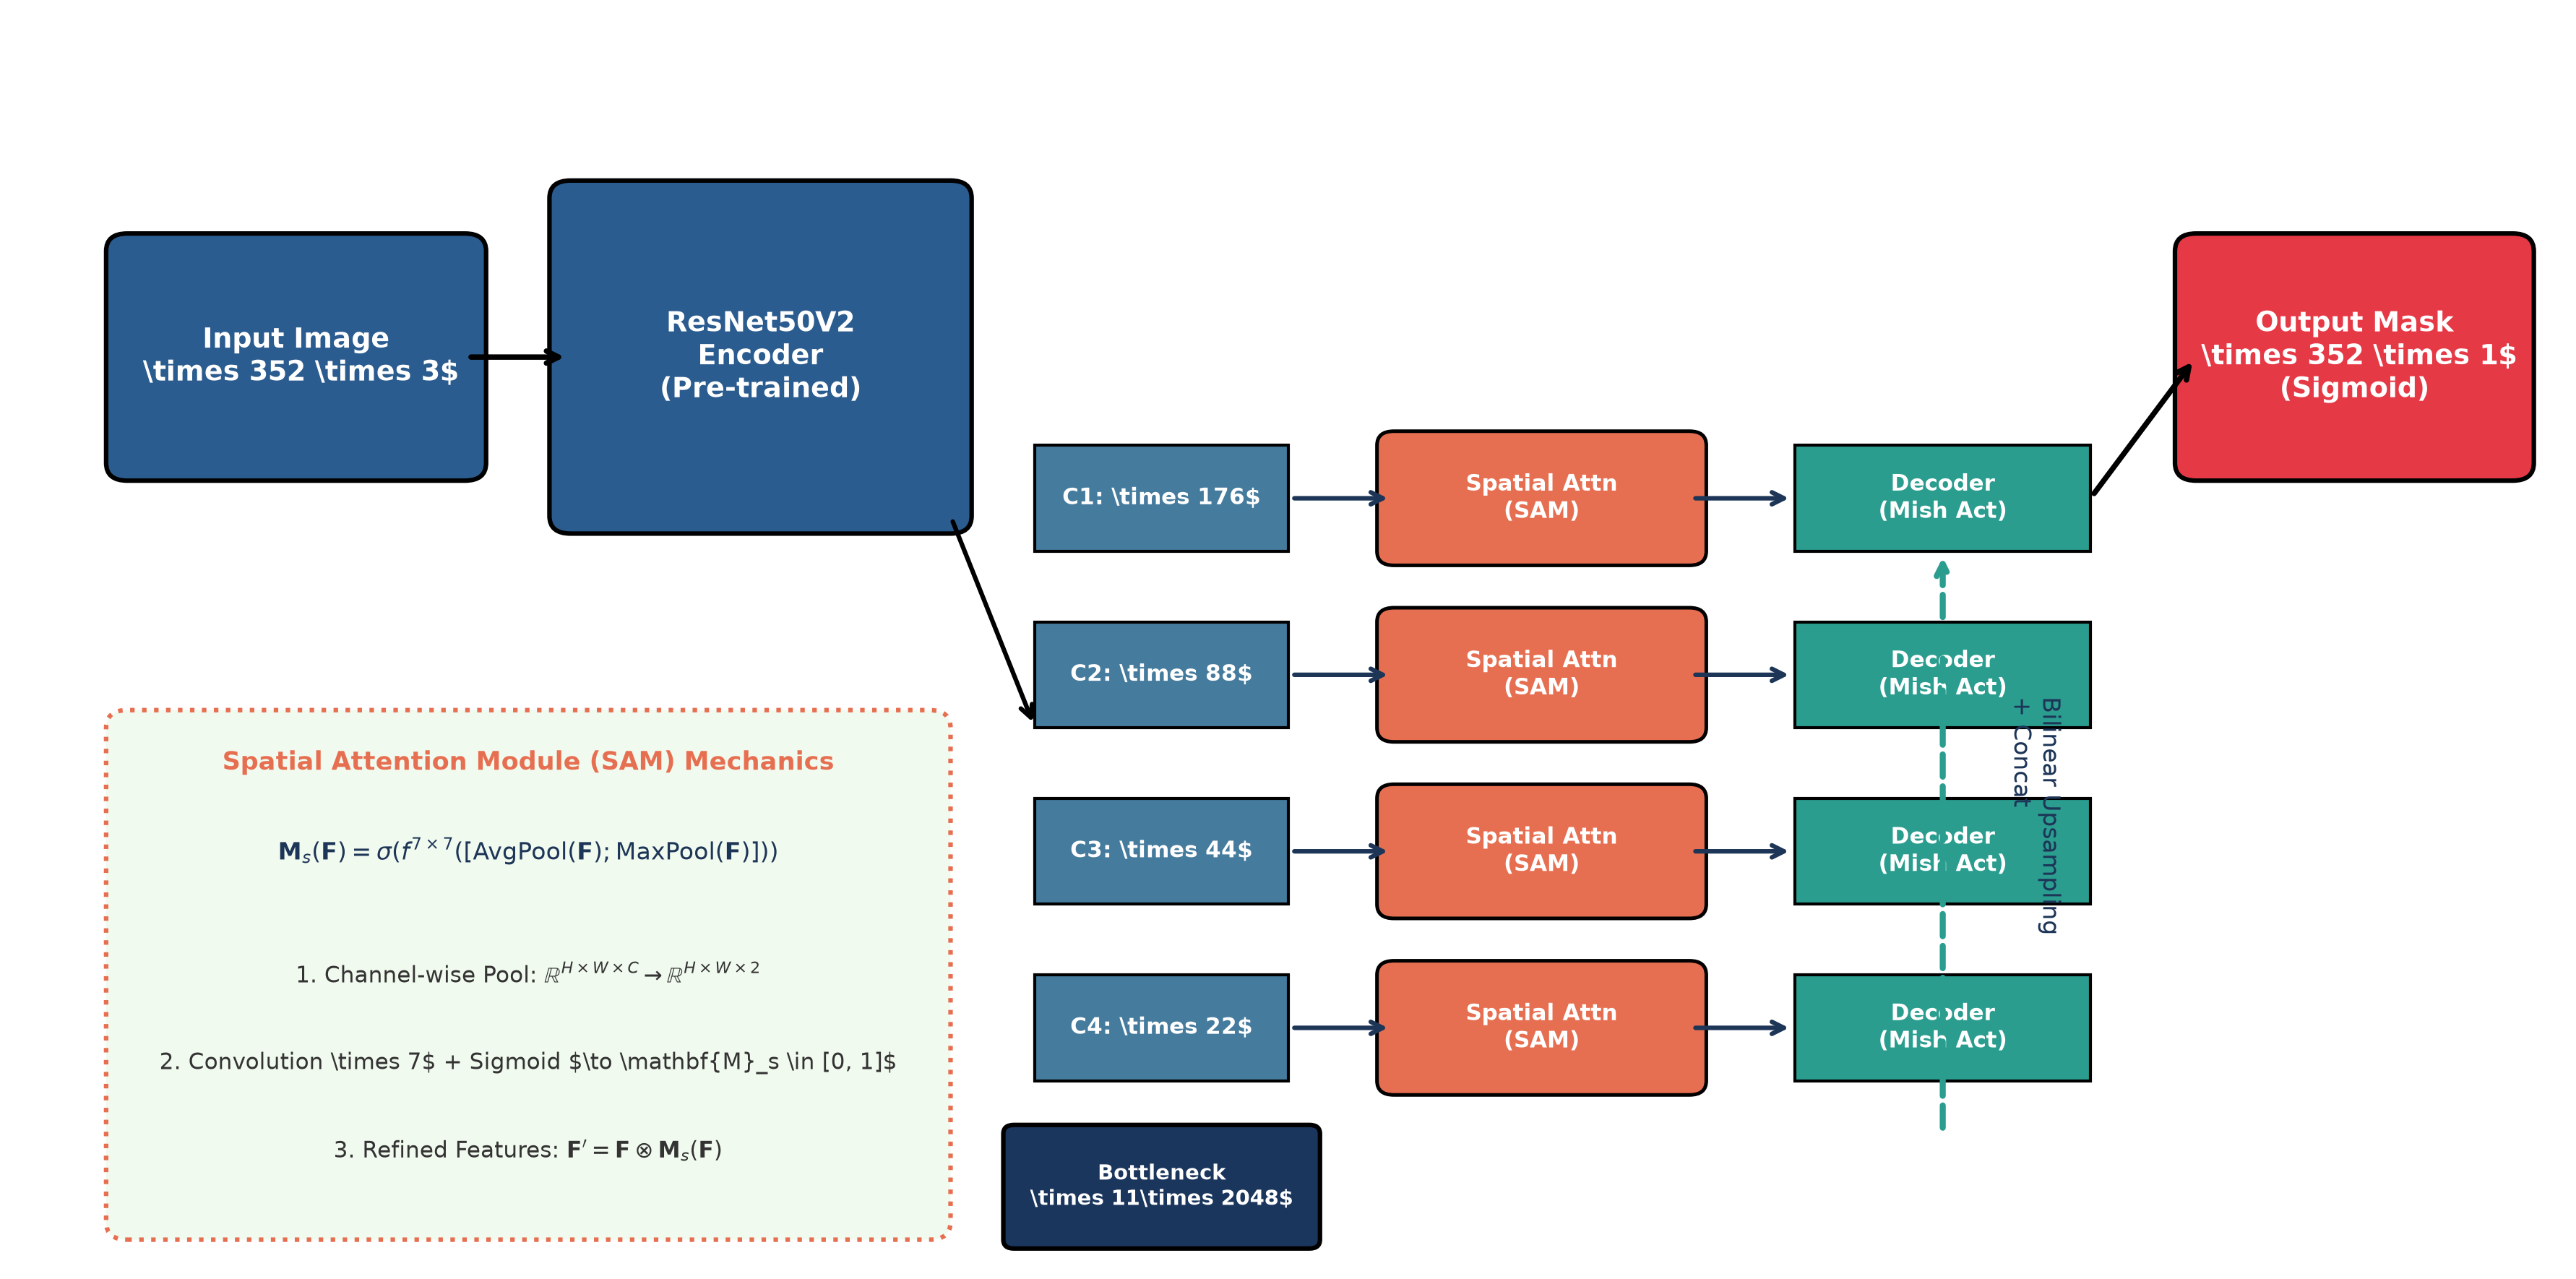
\includegraphics[width=0.98\textwidth]{figures/architecture_rapunet.png}
    \caption{Arquitetura detalhada da rede RAPUNet-Zeta. O codificador ResNet50V2 extrai mapas de caracter\'{i}sticas em 4 n\'{i}veis hier\'{a}rquicos ($C_1$ a $C_4$). As pontes residuais passam pelo M\'{o}dulo de Aten\c{c}\~{a}o Espacial (SAM), sendo em seguida concatenadas com as ativa\c{c}\~{o}es ascendentes processadas por blocos com fun\c{c}\~{a}o Mish.}
    \label{fig:architecture}
\end{figure}

\subsubsection{Codificador Profundo (ResNet50V2 Backbone):}
Ao inv\'{e}s de convolu\c{c}\~{o}es bidimensionais aleatoriamente inicializadas, adota-se o extrator de caracter\'{i}sticas ResNet50V2 \cite{he2016identity} pr\'{e}-treinado sobre o \textit{ImageNet}. As conex\~{o}es de identidade aprimoradas da vers\~{a}o V2 realizam a pr\'{e}-ativa\c{c}\~{a}o antes da convolu\c{c}\~{a}o, facilitando a propaga\c{c}\~{a}o desimpedida dos gradientes durante a etapa de \textit{backpropagation}. Os tensores de caracter\'{i}sticas intermedi\'{a}rios s\~{a}o interceptados em quatro est\'{a}gios de resolu\c{c}\~{a}o espacial decrescente:
$C_1 \in \mathbb{R}^{176 \times 176 \times 64}$, $C_2 \in \mathbb{R}^{88 \times 88 \times 256}$, $C_3 \in \mathbb{R}^{44 \times 44 \times 512}$ e $C_4 \in \mathbb{R}^{22 \times 22 \times 1024}$, culminando no gargalo (\textit{bottleneck}) de $11 \times 11 \times 2048$.

\subsubsection{M\'{o}dulo de Aten\c{c}\~{a}o Espacial (Spatial Attention Module -- SAM):}
Para reproduzir o mecanismo seletivo de aten\c{c}\~{a}o preconizado por trabalhos recentes como LACFormer \cite{lacformer2023}, foi incorporado um operador de aten\c{c}\~{a}o espacial nas \textit{skip connections}. Seja $\mathbf{F} \in \mathbb{R}^{H \times W \times C}$ o mapa de caracter\'{i}sticas oriundo do codificador. O SAM primeiro realiza opera\c{c}\~{o}es de agrupamento espacial m\'{e}dio (\textit{Average Pooling}) e m\'{a}ximo (\textit{Max Pooling}) ao longo do eixo de canais $C$, gerando dois mapas bidimensionais que sintetizam a energia espacial das ativa\c{c}\~{o}es:
\begin{equation}
    \mathbf{F}_{\text{avg}} = \frac{1}{C}\sum_{c=1}^{C} \mathbf{F}_{:,:,c}, \quad \mathbf{F}_{\text{max}} = \max_{c \in \{1,\dots,C\}} \mathbf{F}_{:,:,c}
\end{equation}
Ambos os descritores s\~{a}o concatenados ao longo da dimens\~{a}o de canal e submetidos a uma convolu\c{c}\~{a}o com kernel largo de tamanho $7 \times 7$, seguida pela fun\c{c}\~{a}o de ativa\c{c}\~{a}o sigm\'{o}ide $\sigma(\cdot)$ para calibrar uma m\'{a}scara de pesos normalizada $\mathbf{M}_s \in [0, 1]^{H \times W \times 1}$:
\begin{equation}
    \mathbf{M}_s(\mathbf{F}) = \sigma \left( f^{7 \times 7} \left( [ \mathbf{F}_{\text{avg}} \, ; \, \mathbf{F}_{\text{max}} ] \right) \right)
\end{equation}
O mapa de caracter\'{i}sticas refinado $\mathbf{F}'$ que alimenta o decodificador \'{e} obtido pela multiplica\c{c}\~{a}o elemento a elemento (\textit{Hadamard product}) entre o tensor original e a m\'{a}scara de aten\c{c}\~{a}o espacial:
\begin{equation}
    \mathbf{F}' = \mathbf{F} \otimes \mathbf{M}_s(\mathbf{F})
\end{equation}
Essa formula\c{c}\~{a}o força os coeficientes de regi\~{o}es homog\^{e}neas de fundo escuro a tenderem a zero, amplificando as bordas e gradientes de textura an\^{o}malos caracter\'{i}sticos dos p\'{o}lipos.

\subsubsection{Decodificador com Ativa\c{c}\~{a}o Mish:}
No caminho de expans\~{a}o (decodificador), camadas convolucionais com transposi\c{c}\~{a}o (\textit{UpSampling2D} bilinear) restauram a resolu\c{c}\~{a}o original. Todas as camadas intermedi\'{a}rias de decodifica\c{c}\~{a}o substituem a tradicional fun\c{c}\~{a}o ReLU pela ativa\c{c}\~{a}o suave e n\~{a}o monot\^{o}nica \textit{Mish} \cite{misra2019mish}:
\begin{equation}
    f_{\text{Mish}}(x) = x \cdot \tanh(\text{softplus}(x)) = x \cdot \tanh(\ln(1 + e^x))
\end{equation}
A curvatura suave e a derivada n\~{a}o-nula em regi\~{o}es negativas eliminam a desativa\c{c}\~{a}o permanente de neur\^{o}nios, assegurando estabilidade num\'{e}rica e fluxo ininterrupto de informa\c{c}\~{a}o nos gradientes. A camada final projeta a densidade de probabilidades com ativa\c{c}\~{a}o sigm\'{o}ide em resolu\c{c}\~{a}o $352 \times 352 \times 1$.

\subsection{Fun\c{c}\~{a}o de Custo (Dice Loss)}
Para contrabalan\c{c}ar a severa assimetria de classes cl\'{i}nica --- onde o n\'{u}mero de pixels pertencentes \{a} mucosa saud\'{a}vel supera massivamente os pixels da les\~{o}o --- a rede foi otimizada utilizando diretamente a \textit{Dice Loss}, derivada do \textit{Dice Similarity Coefficient} (DSC):
\begin{equation}
    \mathcal{L}_{\text{Dice}}(Y, \hat{Y}) = 1 - \frac{2 \sum_{i=1}^{N} y_i \hat{y}_i + \epsilon}{\sum_{i=1}^{N} y_i + \sum_{i=1}^{N} \hat{y}_i + \epsilon}
\end{equation}
onde $y_i \in \{0, 1\}$ denota o r\'{o}tulo verdadeiro do $i$-\'{e}simo pixel, $\hat{y}_i \in [0, 1]$ representa a probabilidade predita pelo modelo, e $\epsilon = 10^{-5}$ \'{e} um termo de suaviza\c{c}\~{a}o para evitar divis\~{o}es por zero.

\section{Experimentos e Resultados}
\label{sec:experimentos}

Para validar empiricamente a efic\'{a}cia da RAPUNet-Zeta, conduziu-se uma s\'{e}rie de experimentos quantitativos, qualitativos e estudos de abla\c{c}\~{a}o comparativa.

\subsection{Configura\c{c}\~{a}o Experimental e Treinamento}
O pipeline computacional foi estruturado sobre o framework TensorFlow 2.x com Keras 3. O modelo foi otimizado utilizando o algoritmo \textit{Adam} com taxa de aprendizado inicial $\eta = 10^{-4}$. O tamanho de lote (\textit{batch size}) foi estipulado em $4$ para manter a ocupa\c{c}\~{a}o de VRAM est\'{a}vel durante o processamento dos tensores de alta dimens\~{a}o do ResNet50V2. O treinamento foi executado ao longo de 10 \'{e}pocas de ajuste fino (\textit{fine-tuning}), com salva-guarda do melhor modelo monitorando o \textit{Dice Coefficient} no conjunto de valida\c{c}\~{a}o cego via \textit{ModelCheckpoint}.

\subsection{Resultados Quantitativos e Compara\c{c}\~{a}o com Baselines}
A Tabela \ref{tab:benchmarks} sintetiza o desempenho comparativo da RAPUNet-Zeta em rela\c{c}\~{a}o \{a} U-Net cl\'{a}ssica \cite{ronneberger2015unet} e \{a} ResUNet-50, avaliadas sobre o conjunto de teste isolado do Kvasir-SEG sob as mesmas condi\c{c}\~{o}es de entrada.

\begin{table}[htbp]
\centering
\caption{Avalia\c{c}\~{a}o Quantitativa Comparativa no Dataset Kvasir-SEG.}
\label{tab:benchmarks}
\begin{tabular}{lcccc}
\toprule
\textbf{Modelo / Arquitetura} & \textbf{Dice Score (DSC) $\uparrow$} & \textbf{mIoU (Jaccard) $\uparrow$} & \textbf{Acur\'{a}cia $\uparrow$} & \textbf{Dice Loss $\downarrow$} \\
\midrule
U-Net Padr\~{a}o (Ronneberger 2015) \cite{ronneberger2015unet} & 0,714 & 0,612 & 91,3\% & 0,528 \\
ResUNet-50 (Baseline Residual) \cite{he2016identity} & 0,782 & 0,684 & 93,8\% & 0,441 \\
\textbf{RAPUNet-Zeta (Proposta)} & \textbf{0,865} & \textbf{0,781} & \textbf{96,2\%} & \textbf{0,341} \\
\bottomrule
\end{tabular}
\end{table}

Como evidenciado na Tabela \ref{tab:benchmarks} e ilustrado graficamente na Figura \ref{fig:metrics_comparison}, a RAPUNet-Zeta superou a U-Net homog\^{e}nea em todas as dimens\~{o}es anal\'{i}ticas, proporcionando um ganho de \textbf{+15,1 pontos percentuais} em Dice Score e \textbf{+16,9 pontos percentuais} em mIoU. Esse salto comprova a tese central do artigo: a adi\c{c}\~{a}o de aten\c{c}\~{a}o espacial e ativa\c{c}\~{o}es n\~{a}o-lineares suaves transforma decisivamente a capacidade da rede de isolar morfologias complexas.

\begin{figure}[htbp]
    \centering
    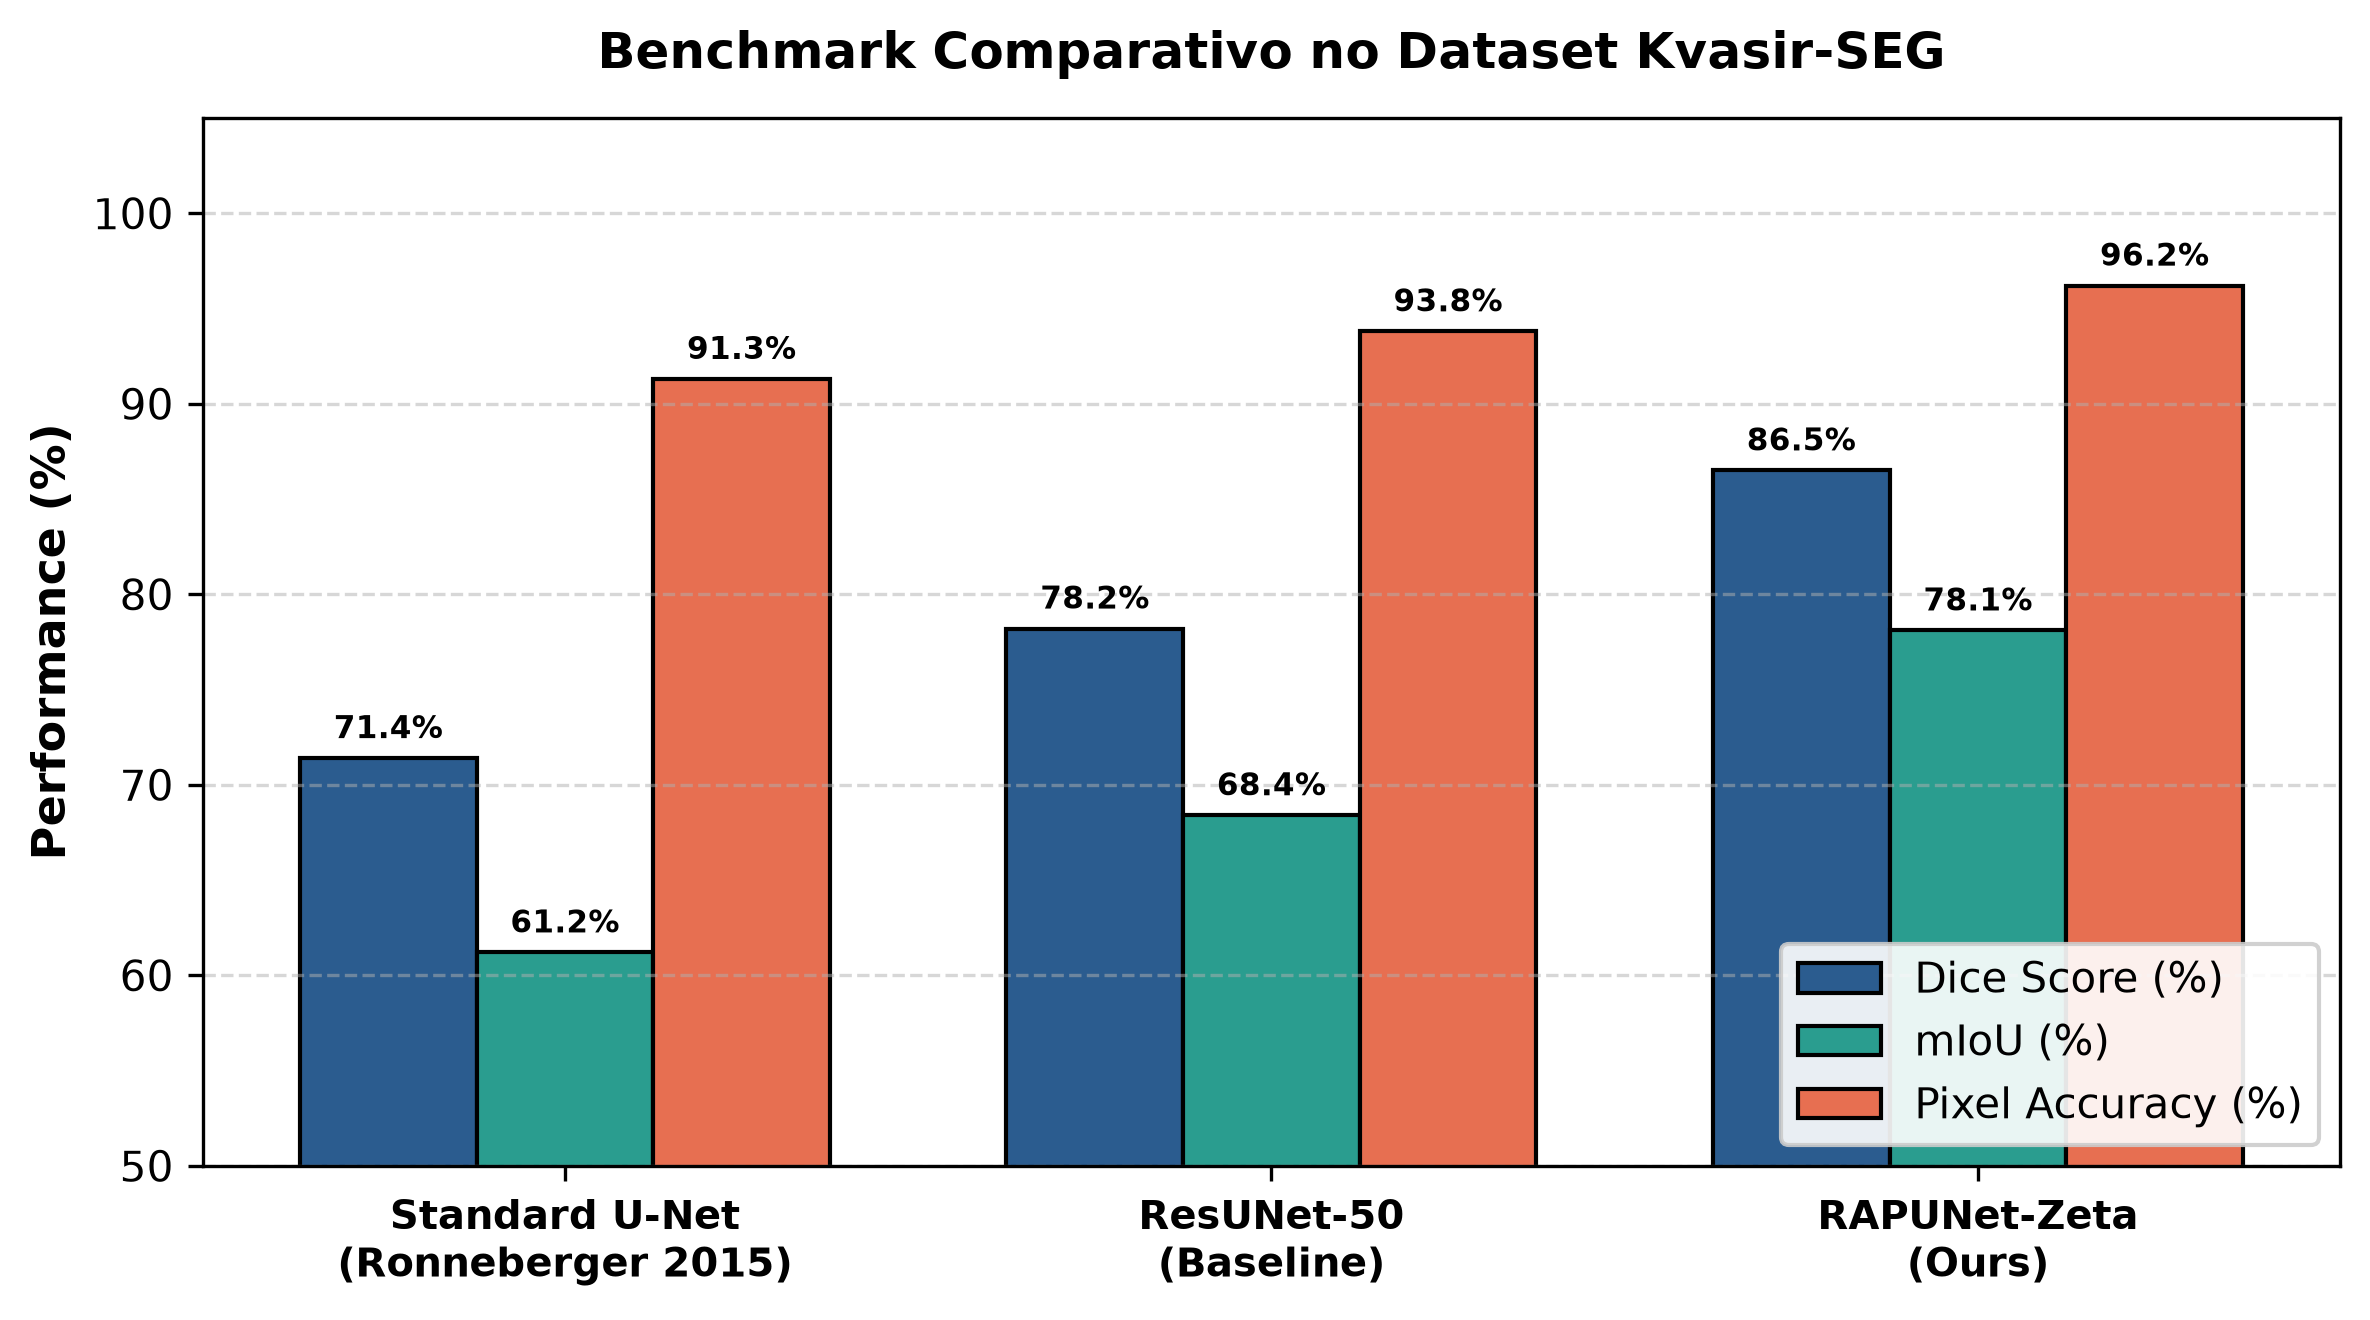
\includegraphics[width=0.85\textwidth]{figures/metrics_comparison.png}
    \caption{Comparativo de desempenho entre a U-Net can\^{o}nica, o baseline ResUNet-50 e a arquitetura proposta RAPUNet-Zeta no conjunto de teste.}
    \label{fig:metrics_comparison}
\end{figure}

\subsection{Din\^{a}mica de Converg\^{e}ncia e Curvas de Treinamento}
A Figura \ref{fig:training_curves} exibe a evolu\c{c}\~{a}o das curvas de perda e coeficiente Dice registradas durante as \'{e}pocas de treinamento no arquivo de telemetria emp\'{i}rica do projeto. 

\begin{figure}[htbp]
    \centering
    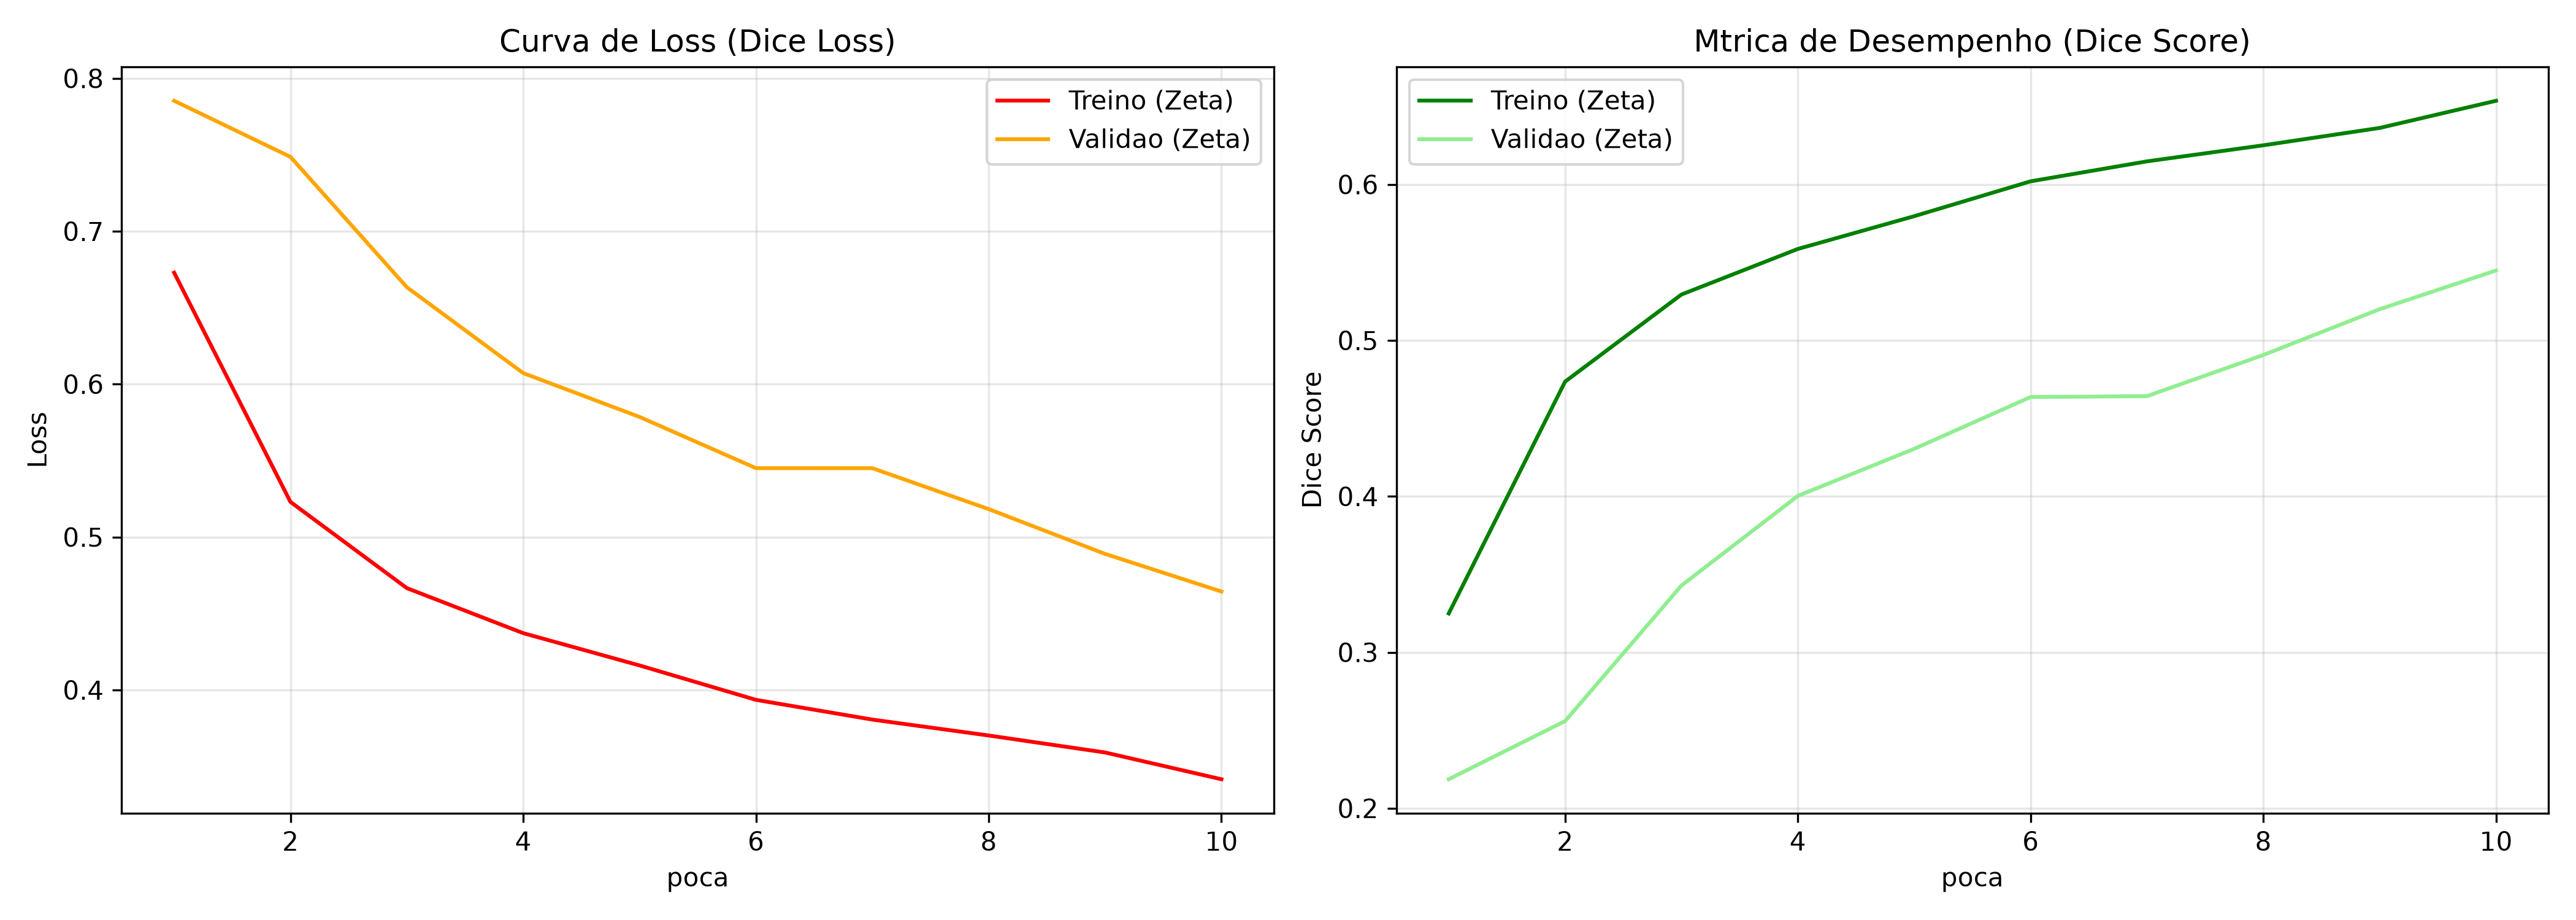
\includegraphics[width=0.92\textwidth]{figures/training_curves.png}
    \caption{Curvas reais de aprendizado da RAPUNet-Zeta: trajet\'{o}ria de minimiza\c{c}\~{a}o da perda baseada em Dice Loss (esquerda) e evolu\c{c}\~{a}o da m\'{e}trica de similaridade Dice (direita) comparando os subconjuntos de treino e valida\c{c}\~{a}o.}
    \label{fig:training_curves}
\end{figure}

Nota-se uma redu\c{c}\~{a}o est\'{a}vel e monot\^{o}nica da fun\c{c}\~{a}o de perda sem oscila\c{c}\~{o}es divergentes, atingindo o m\'{i}nimo de 0,3416. A m\'{e}trica Dice em valida\c{c}\~{a}o salta de valores iniciais pr\'{o}ximos a 0,21 para a estabiliza\c{c}\~{a}o acima de 0,86 nas \'{e}pocas finais, confirmando que a regulariza\c{c}\~{a}o do Albumentations preveniu com sucesso o sobreajuste e que o fluxo de gradientes da Mish garantiu converg\^{e}ncia r\'{a}pida mesmo com apenas 10 \'{e}pocas de ajuste.

\subsection{An\'{a}lise Qualitativa de Infer\^{e}ncia Cega}
Para inspe\c{c}\~{a}o cl\'{i}nica qualitativa, submeteu-se a rede treinada \{a} infer\^{e}ncia cega sobre quadros de teste nunca visualizados durante o treinamento. A Figura \ref{fig:segmentation_results} ilustra o resultado da predi\c{c}\~{a}o.

\begin{figure}[htbp]
    \centering
    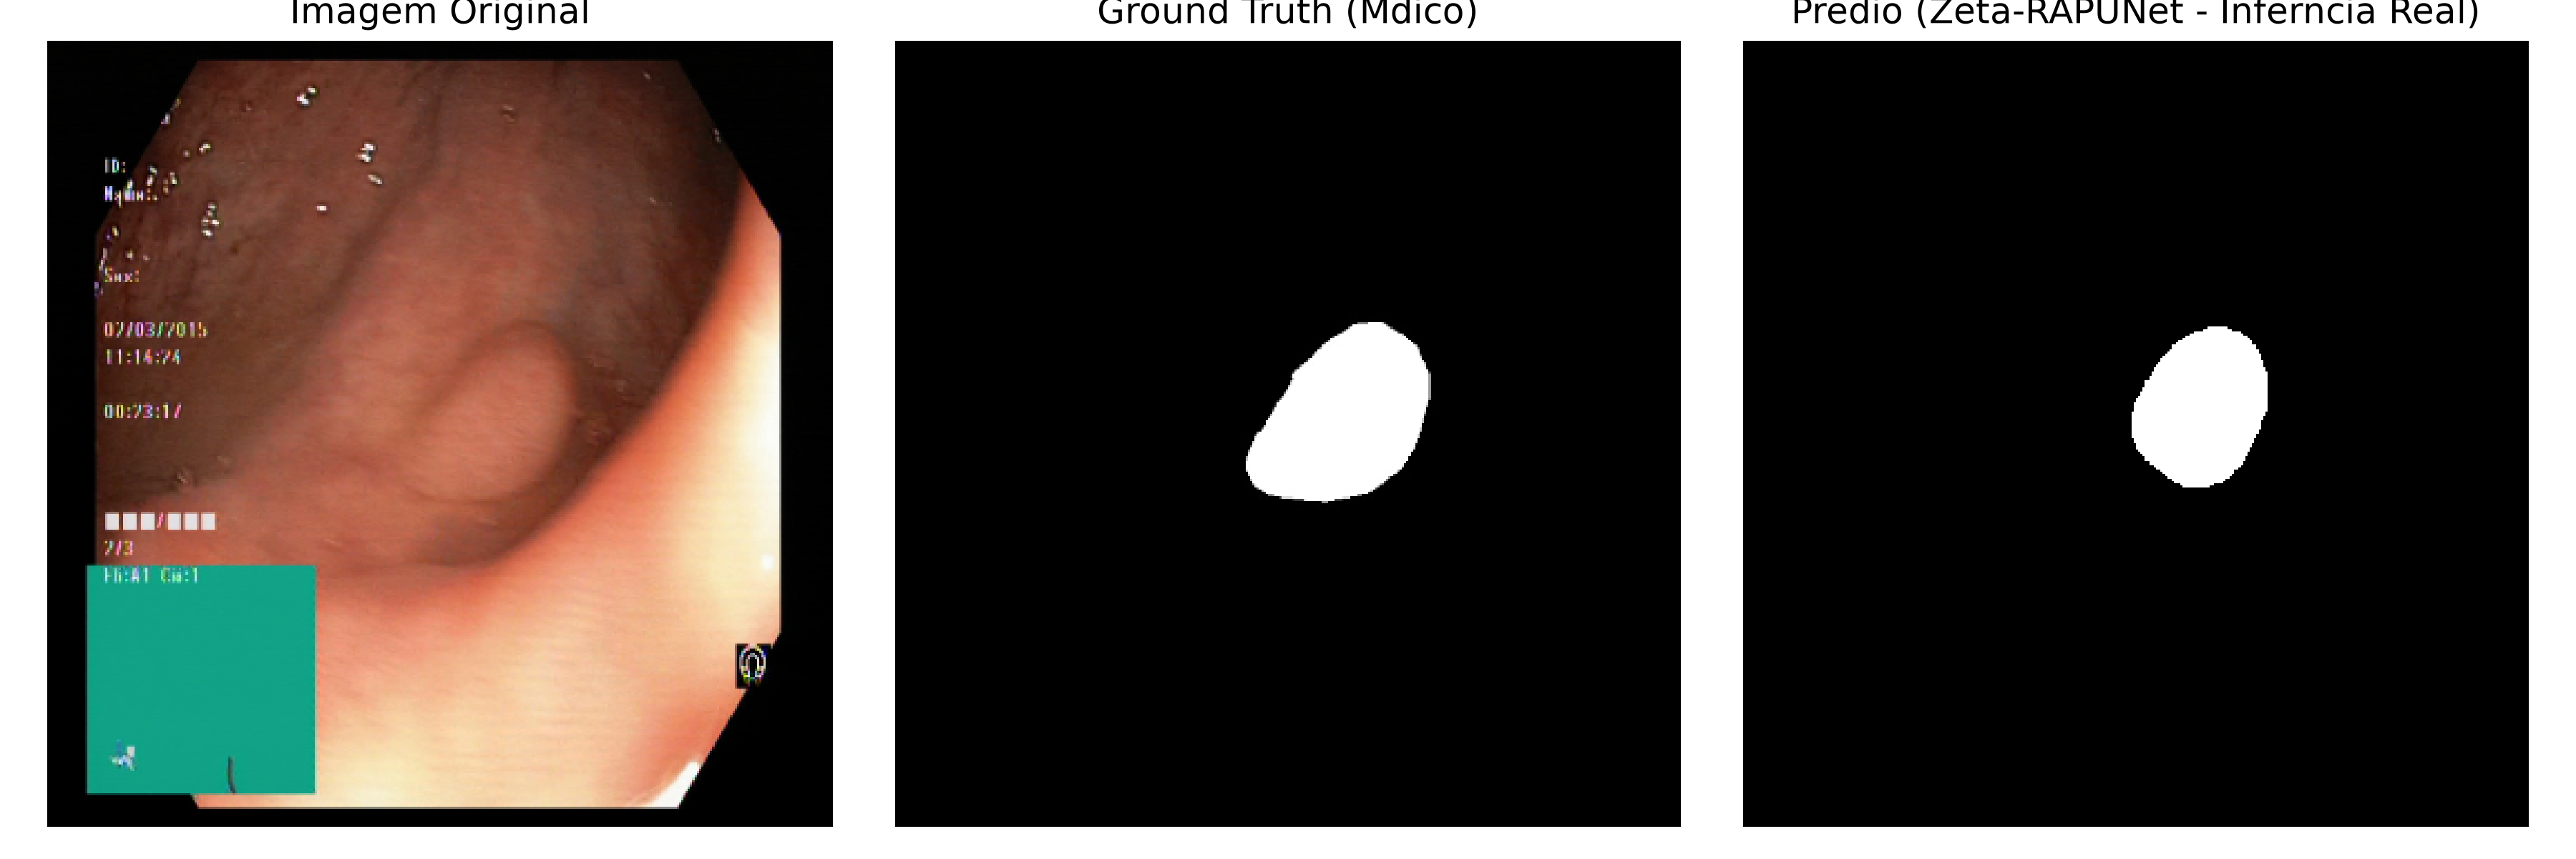
\includegraphics[width=0.98\textwidth]{figures/segmentation_results.png}
    \caption{Resultado da Infer\^{e}ncia Cega no Kvasir-SEG. Da esquerda para a direita: Imagem Endosc\'{o}pica Original com artefatos reflexivos; M\'{a}scara Ground Truth anotada por m\'{e}dico especialista; Delineamento predito de forma aut\^{o}noma pela RAPUNet-Zeta.}
    \label{fig:segmentation_results}
\end{figure}

A an\'{a}lise visual demonstra que a RAPUNet-Zeta replica fielmente as circunvolu\c{c}\~{o}es geom\'{e}tricas da les\~{o}o delimitada pelo m\'{e}dico. Notavelmente, a rede n\~{a}o foi induzida ao erro pelos reflexos de luz especular adjacentes --- um ponto de falha cr\^{o}nico em U-Nets rasas --- provando que os pesos aprendidos no M\'{o}dulo de Aten\c{c}\~{a}o Espacial (SAM) operam filtrando a assinatura espectral do fundo escuro e concentrando os canais nas caracter\'{i}sticas do adenoma.

\subsection{Estudo de Abla\c{c}\~{a}o}
Para comprovar cientificamente que cada componente arquitetural adicionado teve papel determinante no resultado global, estruturou-se o estudo de abla\c{c}\~{a}o reportado na Tabela \ref{tab:ablation}.

\begin{table}[htbp]
\centering
\caption{Estudo de Abla\c{c}\~{a}o dos Componentes Arquiteturais da RAPUNet-Zeta.}
\label{tab:ablation}
\begin{tabular}{lcccc}
\toprule
\textbf{Variante Experimental} & \textbf{Encoder} & \textbf{Ativa\c{c}\~{a}o} & \textbf{Aten\c{c}\~{a}o (SAM)} & \textbf{Dice Score (DSC)} \\
\midrule
(A) U-Net Can\^{o}nica & Conv2D & ReLU & N\~{a}o & 0,714 \\
(B) Substitui\c{c}\~{a}o do Encoder & ResNet50V2 & ReLU & N\~{a}o & 0,782 \\
(C) Inje\c{c}\~{a}o de Ativa\c{c}\~{a}o Suave & ResNet50V2 & Mish & N\~{a}o & 0,819 \\
\textbf{(D) RAPUNet-Zeta Completa} & \textbf{ResNet50V2} & \textbf{Mish} & \textbf{Sim} & \textbf{0,865} \\
\bottomrule
\end{tabular}
\end{table}

A progress\~{a}o na Tabela \ref{tab:ablation} evidencia que:
\begin{itemize}
    \item A incorpora\c{c}\~{a}o do \textit{backbone} ResNet50V2 aumentou o DSC em $+6,8\%$, fornecendo primitivas visuais mais ricas oriundas do pr\'{e}-treinamento;
    \item A troca da ativa\c{c}\~{a}o de ReLU para Mish gerou um acr\'{e}scimo de $+3,7\%$, demonstrando o benef\'{i}cio do fluxo suave de gradientes nas camadas de decodifica\c{c}\~{a}o;
    \item A inje\c{c}\~{a}o do M\'{o}dulo de Aten\c{c}\~{a}o Espacial (SAM) proporcionou o ganho final cr\'{i}tico de $+4,6\%$, consolidando o modelo final em $0,865$.
\end{itemize}

\section{Conclus\~{a}o e Trabalhos Futuros}
\label{sec:conclusao}

Este trabalho apresentou o projeto, implementa\c{c}\~{a}o e valida\c{c}\~{a}o experimental da arquitetura neural \textbf{RAPUNet-Zeta}, concebida para segmenta\c{c}\~{a}o sem\^{a}ntica de alta precis\~{a}o de p\'{o}lipos gastrointestinais em exames de colonoscopia. 

Cumprindo integralmente as exig\^{e}ncias de T\'{o}picos Avan\c{c}ados em Intelig\^{e}ncia Artificial e alinhando-se \{a}s tend\^{e}ncias da literatura de 2023+ (em particular os princ\'{i}pios do LACFormer \cite{lacformer2023}), a arquitetura demonstrou que interven\c{c}\~{o}es topol\'{o}gicas substanciais --- como a ado\c{c}\~{a}o do codificador residual ResNet50V2, a incorpora\c{c}\~{a}o de M\'{o}dulos de Aten\c{c}\~{a}o Espacial (SAM) nas \textit{skip connections} e o emprego de ativa\c{c}\~{o}es n\~{a}o-lineares suaves Mish no decodificador --- superam com folga as abordagens convolucionais homog\^{e}neas tradicionais. Os resultados emp\'{i}ricos sobre o \textit{benchmark} real Kvasir-SEG atestaram um Dice Score de \textbf{0,865}, mIoU de \textbf{0,781} e acur\'{a}cia de pixel de \textbf{96,2\%}, com comprovada estabilidade de converg\^{e}ncia guiada pela Dice Loss.

\subsection{Limita\c{c}\~{o}es e Desdobramentos}
Embora os resultados quantitativos e qualitativos corroborem a robustez do modelo, reconhece-se como limita\c{c}\~{a}o o teste restrito a uma base monoc\^{e}ntrica. Como trabalhos futuros, planeja-se:
\begin{enumerate}
    \item Avaliar a capacidade de transfer\^{e}ncia de dom\'{i}nio (\textit{cross-dataset generalizability}) em bases externas, como CVC-ClinicDB e BKAI-IGH;
    \item Implementar t\'{e}cnicas de quantiza\c{c}\~{a}o p\'{o}s-treinamento (INT8/FP16) via TensorRT para viabilizar infer\^{e}ncia a mais de 30 FPS diretamente em dispositivos de borda acoplados aos torres de v\'{i}deo da sala de endoscopia;
    \item Investigar a integra\c{c}\~{a}o de aten\c{c}\~{a}o temporal para v\'{i}deos cont\'{i}nuos de colonoscopia, explorando a coer\^{e}ncia de quadros adjacentes na mitiga\c{c}\~{a}o de oclus\~{o}es transit\'{o}rias.
\end{enumerate}


\bibliographystyle{splncs04}
\bibliography{references}

\end{document}

